% Options for packages loaded elsewhere
\PassOptionsToPackage{unicode}{hyperref}
\PassOptionsToPackage{hyphens}{url}
%
\documentclass[
]{article}
\usepackage{lmodern}
\usepackage{amssymb,amsmath}
\usepackage{ifxetex,ifluatex}
\ifnum 0\ifxetex 1\fi\ifluatex 1\fi=0 % if pdftex
  \usepackage[T1]{fontenc}
  \usepackage[utf8]{inputenc}
  \usepackage{textcomp} % provide euro and other symbols
\else % if luatex or xetex
  \usepackage{unicode-math}
  \defaultfontfeatures{Scale=MatchLowercase}
  \defaultfontfeatures[\rmfamily]{Ligatures=TeX,Scale=1}
\fi
% Use upquote if available, for straight quotes in verbatim environments
\IfFileExists{upquote.sty}{\usepackage{upquote}}{}
\IfFileExists{microtype.sty}{% use microtype if available
  \usepackage[]{microtype}
  \UseMicrotypeSet[protrusion]{basicmath} % disable protrusion for tt fonts
}{}
\makeatletter
\@ifundefined{KOMAClassName}{% if non-KOMA class
  \IfFileExists{parskip.sty}{%
    \usepackage{parskip}
  }{% else
    \setlength{\parindent}{0pt}
    \setlength{\parskip}{6pt plus 2pt minus 1pt}}
}{% if KOMA class
  \KOMAoptions{parskip=half}}
\makeatother
\usepackage{xcolor}
\IfFileExists{xurl.sty}{\usepackage{xurl}}{} % add URL line breaks if available
\IfFileExists{bookmark.sty}{\usepackage{bookmark}}{\usepackage{hyperref}}
\hypersetup{
  pdftitle={Homework 1 - You Can Be A Baseball Analytics Star Too!},
  hidelinks,
  pdfcreator={LaTeX via pandoc}}
\urlstyle{same} % disable monospaced font for URLs
\usepackage[margin=1in]{geometry}
\usepackage{color}
\usepackage{fancyvrb}
\newcommand{\VerbBar}{|}
\newcommand{\VERB}{\Verb[commandchars=\\\{\}]}
\DefineVerbatimEnvironment{Highlighting}{Verbatim}{commandchars=\\\{\}}
% Add ',fontsize=\small' for more characters per line
\usepackage{framed}
\definecolor{shadecolor}{RGB}{248,248,248}
\newenvironment{Shaded}{\begin{snugshade}}{\end{snugshade}}
\newcommand{\AlertTok}[1]{\textcolor[rgb]{0.94,0.16,0.16}{#1}}
\newcommand{\AnnotationTok}[1]{\textcolor[rgb]{0.56,0.35,0.01}{\textbf{\textit{#1}}}}
\newcommand{\AttributeTok}[1]{\textcolor[rgb]{0.77,0.63,0.00}{#1}}
\newcommand{\BaseNTok}[1]{\textcolor[rgb]{0.00,0.00,0.81}{#1}}
\newcommand{\BuiltInTok}[1]{#1}
\newcommand{\CharTok}[1]{\textcolor[rgb]{0.31,0.60,0.02}{#1}}
\newcommand{\CommentTok}[1]{\textcolor[rgb]{0.56,0.35,0.01}{\textit{#1}}}
\newcommand{\CommentVarTok}[1]{\textcolor[rgb]{0.56,0.35,0.01}{\textbf{\textit{#1}}}}
\newcommand{\ConstantTok}[1]{\textcolor[rgb]{0.00,0.00,0.00}{#1}}
\newcommand{\ControlFlowTok}[1]{\textcolor[rgb]{0.13,0.29,0.53}{\textbf{#1}}}
\newcommand{\DataTypeTok}[1]{\textcolor[rgb]{0.13,0.29,0.53}{#1}}
\newcommand{\DecValTok}[1]{\textcolor[rgb]{0.00,0.00,0.81}{#1}}
\newcommand{\DocumentationTok}[1]{\textcolor[rgb]{0.56,0.35,0.01}{\textbf{\textit{#1}}}}
\newcommand{\ErrorTok}[1]{\textcolor[rgb]{0.64,0.00,0.00}{\textbf{#1}}}
\newcommand{\ExtensionTok}[1]{#1}
\newcommand{\FloatTok}[1]{\textcolor[rgb]{0.00,0.00,0.81}{#1}}
\newcommand{\FunctionTok}[1]{\textcolor[rgb]{0.00,0.00,0.00}{#1}}
\newcommand{\ImportTok}[1]{#1}
\newcommand{\InformationTok}[1]{\textcolor[rgb]{0.56,0.35,0.01}{\textbf{\textit{#1}}}}
\newcommand{\KeywordTok}[1]{\textcolor[rgb]{0.13,0.29,0.53}{\textbf{#1}}}
\newcommand{\NormalTok}[1]{#1}
\newcommand{\OperatorTok}[1]{\textcolor[rgb]{0.81,0.36,0.00}{\textbf{#1}}}
\newcommand{\OtherTok}[1]{\textcolor[rgb]{0.56,0.35,0.01}{#1}}
\newcommand{\PreprocessorTok}[1]{\textcolor[rgb]{0.56,0.35,0.01}{\textit{#1}}}
\newcommand{\RegionMarkerTok}[1]{#1}
\newcommand{\SpecialCharTok}[1]{\textcolor[rgb]{0.00,0.00,0.00}{#1}}
\newcommand{\SpecialStringTok}[1]{\textcolor[rgb]{0.31,0.60,0.02}{#1}}
\newcommand{\StringTok}[1]{\textcolor[rgb]{0.31,0.60,0.02}{#1}}
\newcommand{\VariableTok}[1]{\textcolor[rgb]{0.00,0.00,0.00}{#1}}
\newcommand{\VerbatimStringTok}[1]{\textcolor[rgb]{0.31,0.60,0.02}{#1}}
\newcommand{\WarningTok}[1]{\textcolor[rgb]{0.56,0.35,0.01}{\textbf{\textit{#1}}}}
\usepackage{graphicx,grffile}
\makeatletter
\def\maxwidth{\ifdim\Gin@nat@width>\linewidth\linewidth\else\Gin@nat@width\fi}
\def\maxheight{\ifdim\Gin@nat@height>\textheight\textheight\else\Gin@nat@height\fi}
\makeatother
% Scale images if necessary, so that they will not overflow the page
% margins by default, and it is still possible to overwrite the defaults
% using explicit options in \includegraphics[width, height, ...]{}
\setkeys{Gin}{width=\maxwidth,height=\maxheight,keepaspectratio}
% Set default figure placement to htbp
\makeatletter
\def\fps@figure{htbp}
\makeatother
\setlength{\emergencystretch}{3em} % prevent overfull lines
\providecommand{\tightlist}{%
  \setlength{\itemsep}{0pt}\setlength{\parskip}{0pt}}
\setcounter{secnumdepth}{-\maxdimen} % remove section numbering

\title{Homework 1 - You Can Be A Baseball Analytics Star Too!}
\author{}
\date{\vspace{-2.5em}}

\begin{document}
\maketitle

\hypertarget{the-lahman-package}{%
\subsection{The Lahman Package}\label{the-lahman-package}}

Sean Lahman is an author and journalist, who led the fight to make
sports data open to the public. One of his most famous efforts was
creating an open-source database of baseball data. A version of his
database is in R through the \textbf{Lahman} package. In this homework,
we will practice our skills at making plots! Much of the ``grunt'' work
will be done by me, but you will still have plenty to do and change!!

\hypertarget{loading-packages}{%
\subsection{Loading packages}\label{loading-packages}}

\begin{Shaded}
\begin{Highlighting}[]
\CommentTok{# You may have to install these packages before the document will knit. I have}
\CommentTok{# included the installation lines below but commented out! Get rid of the}
\CommentTok{# hashtags before running. You only have to install the package once, but every}
\CommentTok{# time you knit the document you need to have the library statements because it}
\CommentTok{# opens up a fresh session of R behind the scenes.}

\CommentTok{# install.packages("tidyverse")}
\CommentTok{# install.packages("Lahman")}

\CommentTok{# loading the tidyverse and setting the theme to black-white (it's my favorite theme)}
\KeywordTok{library}\NormalTok{(}\StringTok{"tidyverse"}\NormalTok{);}\KeywordTok{theme_set}\NormalTok{(}\KeywordTok{theme_bw}\NormalTok{())}
\CommentTok{# loading the Lahman package}
\KeywordTok{library}\NormalTok{(}\StringTok{"Lahman"}\NormalTok{)}
\end{Highlighting}
\end{Shaded}

Now that we have everything installed and loaded into R, we can take a
look at all of the datasets in the Lahman package\ldots{} and there are
a lot of them! Running the code \texttt{data(package\ =\ "Lahman")} will
open a list of data sets in the Lahman package. There are 30 datasets in
total! We will focus on the \texttt{Batting} dataset. Here it is below:

\begin{Shaded}
\begin{Highlighting}[]
\CommentTok{# original data is a data frame but tibbles are nicer to work with}
\NormalTok{(batting <-}\StringTok{ }\KeywordTok{as_tibble}\NormalTok{(Batting))}
\end{Highlighting}
\end{Shaded}

\begin{verbatim}
## # A tibble: 105,861 x 22
##    playerID yearID stint teamID lgID      G    AB     R     H   X2B   X3B    HR
##    <chr>     <int> <int> <fct>  <fct> <int> <int> <int> <int> <int> <int> <int>
##  1 abercda~   1871     1 TRO    NA        1     4     0     0     0     0     0
##  2 addybo01   1871     1 RC1    NA       25   118    30    32     6     0     0
##  3 allisar~   1871     1 CL1    NA       29   137    28    40     4     5     0
##  4 allisdo~   1871     1 WS3    NA       27   133    28    44    10     2     2
##  5 ansonca~   1871     1 RC1    NA       25   120    29    39    11     3     0
##  6 armstbo~   1871     1 FW1    NA       12    49     9    11     2     1     0
##  7 barkeal~   1871     1 RC1    NA        1     4     0     1     0     0     0
##  8 barnero~   1871     1 BS1    NA       31   157    66    63    10     9     0
##  9 barrebi~   1871     1 FW1    NA        1     5     1     1     1     0     0
## 10 barrofr~   1871     1 BS1    NA       18    86    13    13     2     1     0
## # ... with 105,851 more rows, and 10 more variables: RBI <int>, SB <int>,
## #   CS <int>, BB <int>, SO <int>, IBB <int>, HBP <int>, SH <int>, SF <int>,
## #   GIDP <int>
\end{verbatim}

\begin{Shaded}
\begin{Highlighting}[]
\CommentTok{# let's look at the range of years we have! }
\NormalTok{batting}\OperatorTok{$}\NormalTok{yearID }\OperatorTok\StringTok{ }\KeywordTok{range}\NormalTok{()}
\end{Highlighting}
\end{Shaded}

\begin{verbatim}
## [1] 1871 2018
\end{verbatim}

\begin{Shaded}
\begin{Highlighting}[]
\CommentTok{# from 1871 to 2018! That's a lot! }
\end{Highlighting}
\end{Shaded}

Notes about the code above:

\begin{itemize}
\tightlist
\item
  parentheses around an assignment statement will print the result
\item
  the \texttt{\$} operator will access the specific variable in the
  tibble
\item
  The \texttt{\%\textgreater{}\%} is called the pipe operator and takes
  the result of the left side and puts it in the first argument of the
  function on the right.
\end{itemize}

That's a lot of data (147 years worth) in there! Let's hone in something
interesting in baseball's past that would be cool to look at! In 1969,
the MLB lowered the pitching mound by 10 inches and shrunk the strike
zone to what it is today. This really benefited the batters and took a
huge advantage away from pitchers. Thus, let's look at batting averages
for those two seasons and see if there is a difference graphically.
Specifically, let's make a side-by-side boxplot to carry out our
comparison. The code below carries out this task (almost!).

Description and comments of the code below:

\begin{itemize}
\tightlist
\item
  This code below is often called a data analysis pipeline because I can
  change the years or the minimum at-bats, and get a whole different
  analysis (here just a plot) without having to re-write any code.
\item
  I also hope that you notice/think this code is pretty readable!
  Without any R knowledge, you could probably tell me what is happening.
  That is what the tidyverse is trying to do!
\item
  Code steps explanation:

  \begin{itemize}
  \tightlist
  \item
    The first step filters the data to only include the years 1968 and
    1969. The \texttt{\textbar{}} represents or and to check equality is
    \texttt{==}. A single \texttt{=} is assigning a value to a variable.
  \item
    The second step changes the \texttt{yearID} variable to be a factor
    (categorical variable) because R will yell at you if year is still a
    numeric value when plotting.
  \item
    The third step filters the dataset so that only players with more
    than 50 at-bats are included. This was a personal choice that you
    can change if you want! It gets rid of some outliers due to players
    only batting a few times that year.
  \item
    The fourth step creates a new variable, \texttt{avg} that holds the
    batting average, because it was not present in the original dataset.
  \end{itemize}
\end{itemize}

\textbf{Problem 1}: The code below doesn't create the side-by-side
boxplot of batting average for the two years mentioned above. You need
to complete the code so that it produces the correct plot! I have
included the ggplot call but you need to choose the right aesthetics and
finish the \texttt{geom\_} call. Make sure to remove the hashtags before
the last \texttt{\%\textgreater{}\%} and the \texttt{ggplot} call or it
won't make the graph.

\begin{Shaded}
\begin{Highlighting}[]
\NormalTok{batting }\OperatorTok\StringTok{ }
\StringTok{    }\KeywordTok{filter}\NormalTok{(yearID }\OperatorTok{==}\StringTok{ }\DecValTok{1968} \OperatorTok{|}\StringTok{ }\NormalTok{yearID }\OperatorTok{==}\StringTok{ }\DecValTok{1969}\NormalTok{) }\OperatorTok
\StringTok{    }\KeywordTok{mutate}\NormalTok{(}\DataTypeTok{yearID =} \KeywordTok{as_factor}\NormalTok{(yearID)) }\OperatorTok\StringTok{ }
\StringTok{    }\KeywordTok{filter}\NormalTok{(AB }\OperatorTok{>}\StringTok{ }\DecValTok{50}\NormalTok{) }\OperatorTok\StringTok{ }
\StringTok{    }\KeywordTok{mutate}\NormalTok{(}\DataTypeTok{avg =}\NormalTok{ H }\OperatorTok{/}\StringTok{ }\NormalTok{AB)  }\OperatorTok\StringTok{ }
\StringTok{    }\KeywordTok{ggplot}\NormalTok{(}\KeywordTok{aes}\NormalTok{(yearID, avg)) }\OperatorTok{+}\StringTok{ }\KeywordTok{geom_boxplot}\NormalTok{()}
\end{Highlighting}
\end{Shaded}

\begin{center}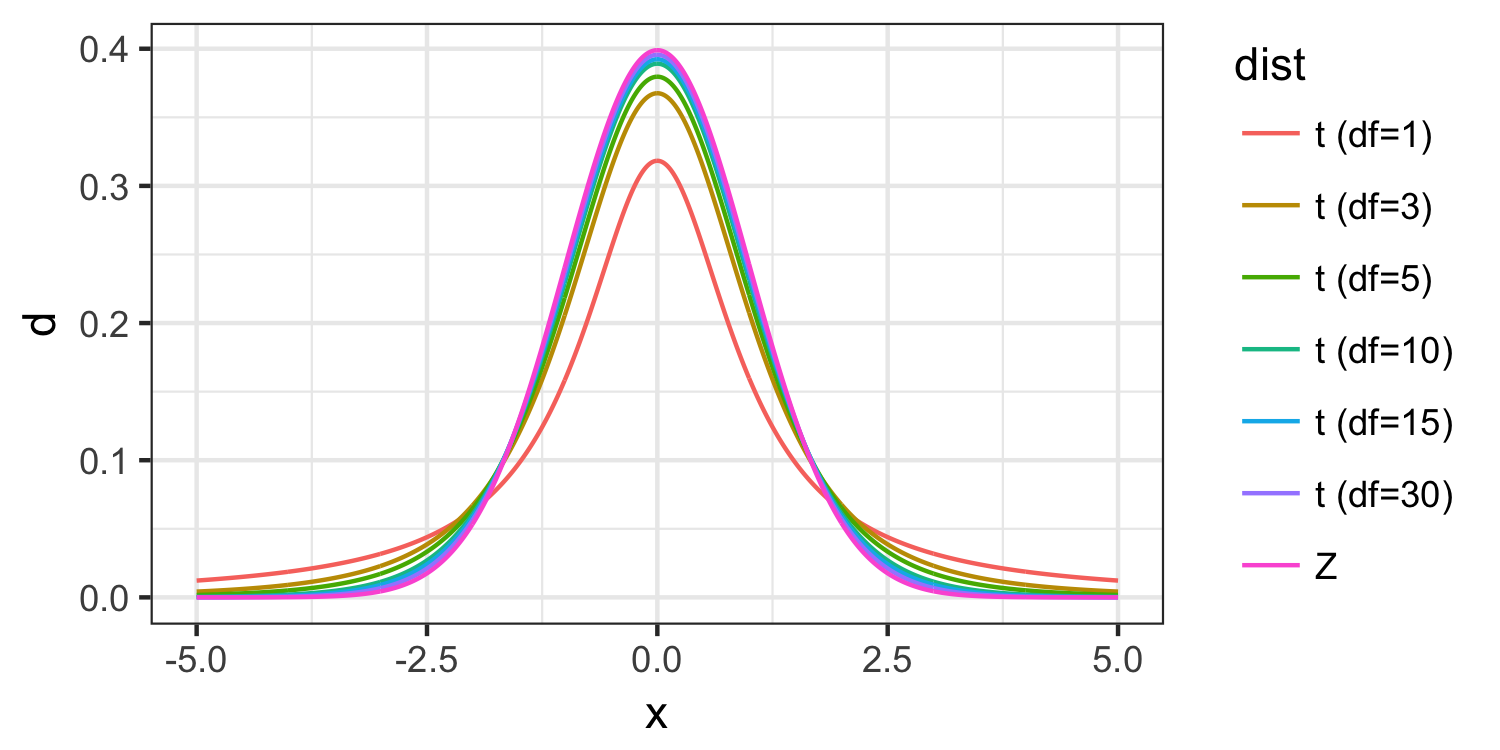
\includegraphics{homework_1_files/figure-latex/unnamed-chunk-3-1} \end{center}

\textbf{Problem 2}: Comment on the plot's findings.

\textbf{Answer:} This is what I found!

Another interesting time in baseball was the steroid era, which I will
define as the 1990's! During this time, an increased number of major
league players used performance enhancing drugs. One way that we could
explore the data to see if there were any side-effects is looking at
home run production. Specifically, I want to make a plot of the total
home run count for every year between 1980 and 2000 with dots and a path
between them. This will give us some reference for before and during the
time when steroids were present. For this plot, I also want to put the
actual home run totals on the plot above the points.

\textbf{Problem 3}: Again, fill in the correct aesthetics that are
missing and the correct geoms to make the points and the path between
them. Again make sure to take away the hashtags to produce the plot.

\begin{Shaded}
\begin{Highlighting}[]
\NormalTok{batting }\OperatorTok\StringTok{ }
\StringTok{    }\KeywordTok{filter}\NormalTok{(yearID }\OperatorTok{>=}\StringTok{ }\DecValTok{1980} \OperatorTok{&}\StringTok{ }\NormalTok{yearID }\OperatorTok{<=}\StringTok{ }\DecValTok{2000}\NormalTok{) }\OperatorTok\StringTok{ }
\StringTok{    }\KeywordTok{group_by}\NormalTok{(yearID) }\OperatorTok\StringTok{ }
\StringTok{    }\KeywordTok{summarize}\NormalTok{(}\DataTypeTok{hr_total =} \KeywordTok{sum}\NormalTok{(HR)) }\CommentTok{# %>% }
\end{Highlighting}
\end{Shaded}

\begin{verbatim}
## # A tibble: 21 x 2
##    yearID hr_total
##     <int>    <int>
##  1   1980     3087
##  2   1981     1781
##  3   1982     3379
##  4   1983     3301
##  5   1984     3258
##  6   1985     3602
##  7   1986     3813
##  8   1987     4458
##  9   1988     3180
## 10   1989     3083
## # ... with 11 more rows
\end{verbatim}

\begin{Shaded}
\begin{Highlighting}[]
     \CommentTok{# ggplot(aes( , , label = hr_total)) + geom_() + geom_() + geom_label(size = 3, vjust = -.25) + labs(x = "Year", y = "Home Run Total")}
\end{Highlighting}
\end{Shaded}

\textbf{Problem 4}: Comment on the plot. Does it seem to support
increased doping in that time span? Do you think any external factors
other than doping could have affected the increase?

One of the most famous players in the doping era was Barry Bonds. Barry
Bonds played for the Pittsburgh Pirates early in his career and was very
successful there, but it wasn't until he started playing for the San
Francisco Giants that he started putting up huge home run numbers. If
you look up ``Barry Bonds Doping'', you will find many pictures of the
difference in body mass between Pittsburgh and in San Francisco. Many
people point to that as evidence toward doping. Let's look at his career
trajectory through his home run production.

\textbf{Problem 5}: I have done the filtering for you, but I want you to
create the entire ggplot by yourself! I have the ggplot call there but
nothing else. Remember to chain ggplot2 statements together with
\texttt{+}'s Do the following:

\begin{itemize}
\tightlist
\item
  Create a point plot of home runs over the years he was active.
\item
  Color the points with the team he was playing for at the time. You'll
  need to add another aesthetic.
\item
  Change the labels to be more descriptive.
\item
  Change the legend so that the legend title says Team and the team name
  is what's describing the color (Pirates, Giants). You will accomplish
  this with the function \texttt{scale\_color\_discrete()}. Make sure to
  look it up for reference.
\end{itemize}

\begin{Shaded}
\begin{Highlighting}[]
\NormalTok{batting }\OperatorTok\StringTok{ }
\StringTok{    }\KeywordTok{filter}\NormalTok{(playerID }\OperatorTok{==}\StringTok{ "bondsba01"}\NormalTok{) }\CommentTok{#%>% }
\end{Highlighting}
\end{Shaded}

\begin{verbatim}
## # A tibble: 22 x 22
##    playerID yearID stint teamID lgID      G    AB     R     H   X2B   X3B    HR
##    <chr>     <int> <int> <fct>  <fct> <int> <int> <int> <int> <int> <int> <int>
##  1 bondsba~   1986     1 PIT    NL      113   413    72    92    26     3    16
##  2 bondsba~   1987     1 PIT    NL      150   551    99   144    34     9    25
##  3 bondsba~   1988     1 PIT    NL      144   538    97   152    30     5    24
##  4 bondsba~   1989     1 PIT    NL      159   580    96   144    34     6    19
##  5 bondsba~   1990     1 PIT    NL      151   519   104   156    32     3    33
##  6 bondsba~   1991     1 PIT    NL      153   510    95   149    28     5    25
##  7 bondsba~   1992     1 PIT    NL      140   473   109   147    36     5    34
##  8 bondsba~   1993     1 SFN    NL      159   539   129   181    38     4    46
##  9 bondsba~   1994     1 SFN    NL      112   391    89   122    18     1    37
## 10 bondsba~   1995     1 SFN    NL      144   506   109   149    30     7    33
## # ... with 12 more rows, and 10 more variables: RBI <int>, SB <int>, CS <int>,
## #   BB <int>, SO <int>, IBB <int>, HBP <int>, SH <int>, SF <int>, GIDP <int>
\end{verbatim}

\begin{Shaded}
\begin{Highlighting}[]
    \CommentTok{# ggplot() +  }
\end{Highlighting}
\end{Shaded}

\textbf{Problem 6}: Comment on the plot.

For this last plot, I want you to think of your favorite baseball
player. If you don't have one or don't care about baseball, then search
for the list of the greatest baseball hitters of all time and choose
from one of those. We are going to plot their batting average over time
and compare it to every other player in the \texttt{Batting} dataset!
Specifically, we are going to do the following:

\begin{itemize}
\tightlist
\item
  Search for the \texttt{playerID} of your person.
\item
  Create a separate dataset just for them and make the batting average
  variable.
\item
  Create a dataset for everyone else that only contains batting averages
  for seasons with more than 50 at-bats. Also, we need to standardize
  the years so that they all fit on one plot.
\item
  Plot the averages over the career years with a line in the background.
\item
  Overlay your favorite players in red.
\end{itemize}

To find your player, we need to look in the \texttt{Master} dataset that
contains personal information about them. For instance, if I was looking
for a player named Roberto Clemente, I would do the following:

\begin{Shaded}
\begin{Highlighting}[]
\KeywordTok{filter}\NormalTok{(Master, nameLast }\OperatorTok{==}\StringTok{ "Clemente"}\NormalTok{)}
\end{Highlighting}
\end{Shaded}

\begin{verbatim}
##    playerID birthYear birthMonth birthDay birthCountry birthState birthCity
## 1 clemeed02      1975         12       15         P.R.       <NA>  Santurce
## 2 clemero01      1934          8       18         P.R.       <NA>  Carolina
##   deathYear deathMonth deathDay deathCountry deathState deathCity nameFirst
## 1        NA         NA       NA         <NA>       <NA>      <NA>    Edgard
## 2      1972         12       31         P.R.       <NA>  San Juan   Roberto
##   nameLast               nameGiven weight height bats throws      debut
## 1 Clemente Edgard Alexis Velazquez    188     71    R      R 1998-09-10
## 2 Clemente                 Roberto    175     71    R      R 1955-04-17
##    finalGame  retroID   bbrefID  deathDate  birthDate
## 1 2000-07-31 cleme001 clemeed02       <NA> 1975-12-15
## 2 1972-10-03 clemr101 clemero01 1972-12-31 1934-08-18
\end{verbatim}

Next, make a dataset with just that player. Also, add two new variables.
One is the batting average and two is the career years that the person
played. For instance, if I were to make one for Roberto, it would look
like this:

\begin{Shaded}
\begin{Highlighting}[]
\NormalTok{clem_bat <-}\StringTok{ }\NormalTok{batting }\OperatorTok\StringTok{ }
\StringTok{    }\KeywordTok{filter}\NormalTok{(playerID }\OperatorTok{==}\StringTok{ "clemero01"}\NormalTok{) }\OperatorTok\StringTok{ }
\StringTok{    }\KeywordTok{mutate}\NormalTok{(}\DataTypeTok{avg =}\NormalTok{ H }\OperatorTok{/}\StringTok{ }\NormalTok{AB, }\DataTypeTok{career =}\NormalTok{ yearID }\OperatorTok{-}\StringTok{ }\KeywordTok{min}\NormalTok{(yearID))}
\end{Highlighting}
\end{Shaded}

Now we are going to do the same thing for everyone else, and add in the
more than 50 AB condition!

\begin{Shaded}
\begin{Highlighting}[]
\NormalTok{other_bats <-}\StringTok{ }\NormalTok{batting }\OperatorTok\StringTok{ }
\StringTok{    }\KeywordTok{filter}\NormalTok{(AB }\OperatorTok{>}\StringTok{ }\DecValTok{50}\NormalTok{) }\OperatorTok\StringTok{ }
\StringTok{    }\KeywordTok{group_by}\NormalTok{(playerID) }\OperatorTok\StringTok{ }
\StringTok{    }\KeywordTok{arrange}\NormalTok{(playerID, yearID, teamID) }\OperatorTok
\StringTok{    }\KeywordTok{mutate}\NormalTok{(}\DataTypeTok{avg =}\NormalTok{ H }\OperatorTok{/}\StringTok{ }\NormalTok{AB, }\DataTypeTok{career =}\NormalTok{ yearID }\OperatorTok{-}\StringTok{ }\KeywordTok{min}\NormalTok{(yearID))}
\end{Highlighting}
\end{Shaded}

Lastly, we need to make the plot! Here are the steps you should follow
to make the plot:

\textbf{Problem 7}:

\begin{itemize}
\tightlist
\item
  First call \texttt{ggplot()} using the \texttt{other\_bats} data with
  aesthetics to show change in batting average over time.
\item
  Add on a geom that tracks the path from one year to another. Don't use
  dots. In your call to the geom, make sure to add the statement
  \texttt{alpha\ =\ 0.02}. This is called alpha blending and it help you
  avoid overplotting!
\item
  Make the x axis go from 0 to 20 by 5 and the y axis go from 0 to 0.4
  by 0.1. This is accomplished by adding the two lines
  \texttt{scale\_x\_continuous("Career\ Year",\ breaks\ =\ seq(0,\ 20,\ 5),\ limits\ =\ c(0,\ 20))}
  and
  \texttt{scale\_y\_continuous("Batting\ Average",\ breaks\ =\ seq(0,\ 0.4,\ 0.1),\ limits\ =\ c(0,\ 0.4))}.
  This will also fix the labels.
\item
  Lastly, make another line/path using just the data from your player's
  small dataset and color it red.
\end{itemize}

Put the code in the empty code chunk below.

\textbf{Extra Credit}: If you are really interested in making these
plots, I challenge you to try and recreate the plot below about Pete
Rose.

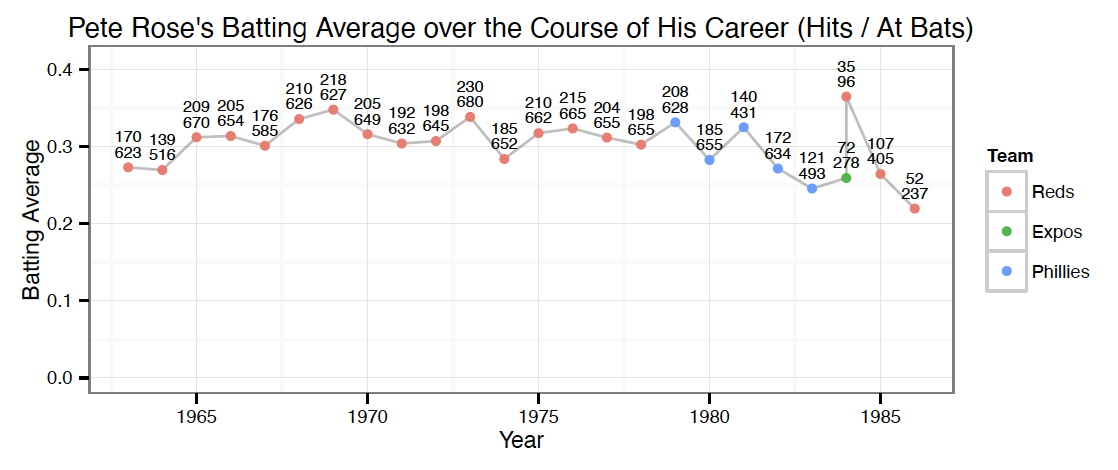
\includegraphics{img/pete_rose_pic.png}

\end{document}
